\begin{figure*}[htb!]
  \includegraphics[width = \textwidth]{figures/reconstructions/1}
  
%  \includegraphics[width = \textwidth]{figures/reconstructions/2}

%   \includegraphics[width = \textwidth]{figures/reconstructions/4} 
 
 \includegraphics[width = \textwidth]{figures/reconstructions/5}    
 
% \includegraphics[width = \textwidth]{figures/reconstructions/28}
 
\includegraphics[width = \textwidth]{figures/reconstructions/29}

 \includegraphics[width = \textwidth]{figures/reconstructions/7}
  
% \includegraphics[width = \textwidth]{figures/reconstructions/8}

   \includegraphics[width = \textwidth]{figures/reconstructions/10}
  
% \includegraphics[width = \textwidth]{figures/reconstructions/11}

 %  \includegraphics[width = \textwidth]{figures/reconstructions/13}
  
 \includegraphics[width = \textwidth]{figures/reconstructions/14}
 \includegraphics[width = \textwidth]{figures/reconstructions/16}
       
%\includegraphics[width = \textwidth]{figures/reconstructions/17}
%\end{figure}
%\begin{figure}
%\includegraphics[width = \textwidth]{figures/reconstructions/19}

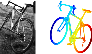
\includegraphics[width = \textwidth]{figures/reconstructions/20}

%
\includegraphics[width = \textwidth]{figures/reconstructions/22}

\includegraphics[width = \textwidth]{figures/reconstructions/23}

\includegraphics[width = \textwidth]{figures/reconstructions/25}

%\includegraphics[width = \textwidth]{figures/reconstructions/26}

\caption{\label{fig:recons}Example reconstructions of objects shown on the left column. Columns 3 and 4 show the 3D reconstruction obtained using our basis shape model and columns 6 and 7 show the one obtained using our prototype shape model. Columns 2 and 5 show the corresponding final depth maps combining both top-down and bottom-up cues. Blue is closer to the camera, red is farther away.}
\end{figure*}